\chapter{Future nEDM Measurement at TRIUMF}

Finding a non-zero neutron EDM is directly linked to the extra sources
of CP violation beyond the standard model. The TUCAN collaboration
proposes a world-leading experiment to measure the nEDM, improving the
precision by a factor of thirty compared to the present world’s best
experimental result. The current nEDM experiments suffer from low UCN
statistics. As a result, TUCAN has intended to build the strongest UCN
source in the world. To achieve this goal extensive studies of the
current vertical UCN source have been conducted~(See
Chapters~\ref{chap:UCNattriumf} and ~\ref{chap:UCNresult}).

To measure the neutron EDM, an ensemble of polarized UCN are put in
the presence of aligned electric and magnetic fields. The hamiltonian
of the interaction of the UCN with electric and magnetic fields are
described in Eqn.~\ref{eqn:hamiltonian}.  The larmor precession
frequency of UCN is then measured in two oriantations of parallel and
anti-parallel electric and magnetic fields. For the parallel $\bf{E}$
and $\bf{B}$ fields the Larmor precession frequency of UCN is written
as
\begin{equation}
\label{eqn:parallelEandB}
  h \nu_{\uparrow \uparrow} = 2 \mu_n \vert {\bf{B^{\uparrow \uparrow}}} \vert+ 2 d_n\vert \bf{ E^{\uparrow \uparrow}} \vert
\end{equation}
and for anti-parallel  $\bf{E}$ and $\bf{B}$ fields it is
\begin{equation}
\label{eqn:antiparallelEandB}
  h \nu_{\uparrow \downarrow} = 2 \mu_n \vert {\bf{B^{\uparrow \downarrow}}} \vert+ 2 d_n\vert \bf{ E^{\uparrow \downarrow}} \vert.
\end{equation}
Here $\uparrow \uparrow$ indicates the parallel Electric and Magnetic
fields and $\uparrow \downarrow$ represent the anti-parallel
orientation of those fields.
A nonzero nEDM is then extracted from any frequecy shift between these
two measurements:
\begin{equation}
  \label{eqn:dn}
  d_n = \frac{h \left( \nu_{\uparrow \uparrow} - \nu_{\uparrow \downarrow} \right) - 2 \mu_n \left( \vert {\bf{B^{\uparrow \uparrow}}} \vert -\vert {\bf{B^{\uparrow \downarrow}}} \vert \right)}{2 \left(\vert \bf{ E^{\uparrow \uparrow}} \vert - \vert \bf{ E^{\uparrow \downarrow}} \vert \right)}
\end{equation}
The main reason to employ this method is because it is impossible to
completely eliminate the $\bf{B}$ field to extract the neutron
EDM. These measurements are either performed in two adjacent volumes
with
$\vert E^{\uparrow \uparrow} \vert = - \vert E^{\uparrow \downarrow}
\vert$ and
$\vert B^{\uparrow \uparrow}\vert - \vert B^{\uparrow \downarrow} = 0
$ or measured in the same volume where the configuration of the fields
change in time. In the first case it is essential to make sure that
the magnetic field inside both volumes are the same and there is no
field gradient and in the second method it is essential to make sure
that the magnetic field is stable in time.

\subsubsection{Ramsey Method of Separated Oscillating
  Fields\label{sec:Ramsey}}

The Ramsey method of separated oscillating fields is the well-known
measurement technique to extract the neutron EDM. Ramsey obtained an
expression for the quantum mechanical transition probability of a
system between two states when the system subjected to such separated
oscillating
fields~\cite{ramsey1950}. Fig.~\ref{fig:ramsey}~\cite{Schmidt2016} left
shows a cycle of measurement. An ensemble of polarized UCN with the
inital spin $\ket{ \uparrow}$ are exposed to a DC magnetic field of
$B_0$.  A first RF pulse of $B_1 \cos (\omega_{rf}t)$ prependicular to
the $B_0$ field tips the spin of the neutrons to the transverse
plane. The neutrons precess freely with their Larmor precession
frequency $\omega_0$ for some time $T$ while accumulating a phase of
$\phi = \gamma_n BT$. Then again the second oscillating magnetic field
pulse of $B_1 \cos (\omega_{rf}t)$ is applied to the neutron
ensemble. The essential idea is to compare the phase $\phi$ with
$\omega_{rf}T$ and if they are identical then
$B= \omega_{rf} / \gamma_n$.

\begin{figure}[h]
  \centering
  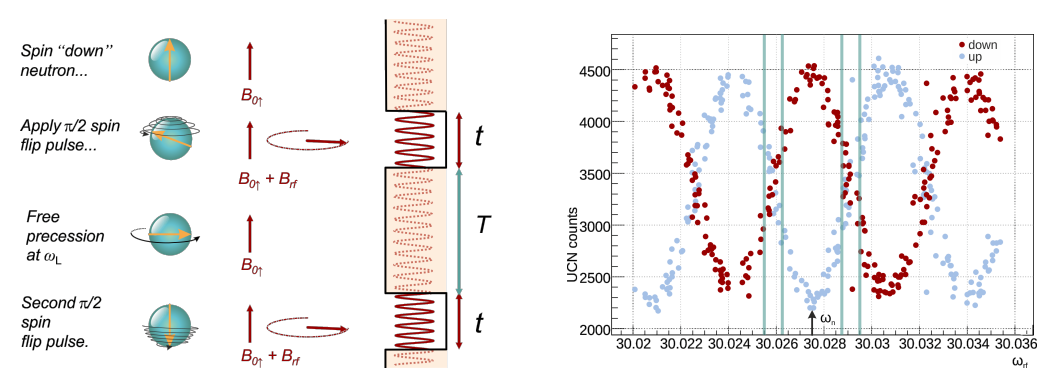
\includegraphics[width=1.0\textwidth]{ramsey.png}
  \caption{Ramsey method of separated oscillating fields. Left shows
    the scheme of a measurement procedure and right shows the data
    points. The blue points are the UCN counts with the spin up and
    the red points are the UCN with spin down (data from the PSI-nEDM
    collaboration). The width at half height~$\Delta \nu$ of the
    central fringe is approximately $1/2T$, the four vertical lines
    indicate the working points.}
  \label{fig:ramsey}
\end{figure}

The probability to find the UCN with spin up is
\begin{equation}
  \label{eqn:spinup}
  P(T, \omega_{rf}) = \bra{\uparrow} U(T, \omega_{rf}) \ket{\uparrow}
  = 1 - \frac{4 \omega_1^2}{\Omega^2} \sin ^2 \frac{\Omega t_{\pi/2}}{2} \left[ \frac{\Delta}{\Omega} \sin  \frac{\Omega t_{\pi/2}}{2} \sin \frac{T\Delta}{2} - \cos  \frac{\Omega t_{\pi/2}}{2} \cos\frac{T\Delta}{2} \right]^2,
\end{equation}
where $U(T, \omega_{rf})$ is the time evolutions operator,
$\omega_1 = - \gamma_n B_1$, $\Delta = \omega_{rf} - \omega_0$, and
$\Omega = \sqrt{\Delta^2 + \omega_1^2}$. When the spin-flipping pulses
are optimized we would have $\gamma_n B_1 t_{\pi/2} = \pi / 2$. In
this case the central fringe range ($\Delta \ll \omega_1$) and
Eqn.~\ref{eqn:spinup} simplifies to
\begin{equation}
  P(T, \omega_{rf}) = \frac{1}{2} \left( 1 - \cos(T\Delta) \right).
\end{equation}
In a real measurement with $N$ UCN inside a magnetic field region this becomes
\begin{equation}
  \label{eqn:Nup}
N^{\uparrow} = \frac{N}{2} \left\lbrace 1 - \alpha(T) \cos \left[ (\omega_{rf} - \gamma_n B_0 ) \cdot \left(T+\frac{T+4t_{\pi/2}}{\pi}\right)\right]\right\rbrace,
\end{equation}
where $\alpha$ is the visibility of the central fringe with spin either up or down
\begin{equation}
  \label{eqn:visibility}
  \alpha^{\uparrow /\downarrow} = \frac{N_{max}^{\uparrow /\downarrow} - N_{min}^{\uparrow /\downarrow}}{N_{max}^{\uparrow /\downarrow}+ N_{min}^{\uparrow /\downarrow}}.
\end{equation}
The term $4t_{\pi/2}/\pi$ is necessary to account for field
inhomogeneities of $B_1$ and $B_0$ which become relevant when the
pulse lenght $t_{\pi/2}$ is finite. The graph in Fig.~\ref{fig:ramsey}
shows the Ramsey interference pattern by scanning $\omega_{rf}$ while
everything else is kept the same. In actual nEDM measurements, only 4
points with the highest sensitivity are measured. These points are
refered to as the working points. For each configuration of the
electric and magnetic fields (parallel or anti-parallel)
Eqn.~\ref{eqn:Nup} is fitted to the data to extract the Larmor
frequency. Taking the differences of those Larmor frequencies then
give access to the neutron EDM
\begin{equation}
  \label{eqn:fitteddn}
  d_n = \frac{\hbar (\omega_0 ^{\uparrow \uparrow} - \omega_0 ^{\uparrow \downarrow})}{2(E^{\uparrow \uparrow} - E^{\uparrow \downarrow})} = \frac{\hbar \Delta \omega}{4E}.
\end{equation}
with the assumption that the magnetic field is constant~(See
Eqn.~\ref{eqn:dn}).
The statistical sensitivity of nEDM measurement is
\begin{equation}
  \label{eqn:dnsensitivity}
\sigma(d_n) = \frac{\hbar}{2 \alpha T E \sqrt{\bar{N}}}
\end{equation}
where $\bar{N}$ is the average total number of detected UCN.

Fig.~\ref{fig:triumfEDM} shows the top view of the future EDM facility
at TRIUMF.

\begin{figure}[h]
  \centering
  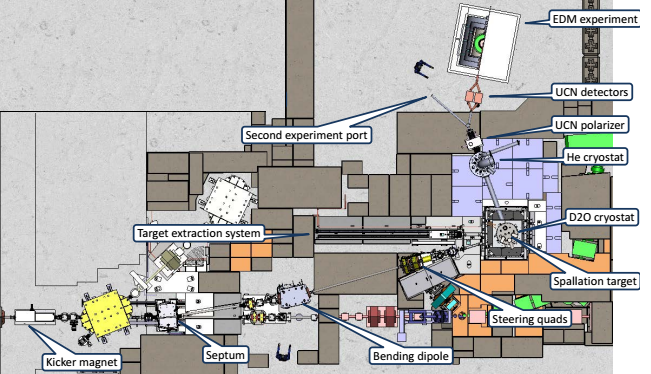
\includegraphics[width=1.0\textwidth]{topview.png}
  \caption{}
  \label{fig:triumfEDM}
\end{figure}


%Based on the previous measurements of nEDM, the dominant systematic
%uncertainty is due to the magnetic field insability and
%inhomogeneity. As a result, different types of magnetic shielding is
%needed to meet the magnetic requirements.

% For after I am back
% I can use the old CDR and my thesis proposal to write some components
% I can use another CDR to write about high voltage and stuff



\section{Magnetic Stability Requirements}
\subsection{Active Shielding}

\subsection{Magnetically Shielded room}

\subsection{Passive Shielding}


\section{High Voltage EDM Cells}

\section{Dual Comagnetometer}



\begin{description}
\item{An introduction about the long term nEDM effort at TRIUMF, what
  the plan is, when it will start (roughly). I guess I can probably
  get this information from some proposals. I am not sure how much
  detail should go here.}
  
\item{How the EDM experiment is actually done, talk about different
  components of the system. Here is where I talk about the Ramsey
  cycle ...}
  
\item{nEDM measurement systematic effects: This is where I talk about
  the GPE and ... . Basically here is to kind of motivate that we need
  to have stable magnetic fields and we need lots of neutrons.}
  
\item{Introduction to the magnetic stability requirements at
  TRIUMF. What I mean is that there is 400 $\mu$T background field at
  TRIUMF. Hopefully we have a field map of the area soon(?).}
  
\item{From ouside in: Magnetically shielded room, what is the status
  of that, are we going to have it? when? How good is it going to be
  compared to the other ones worldwide? Why is it designed that way?
  What is the design? Drawings of it. General question: Some of these
  are about things that will happen in the future and I have not
  worked on them. Should they even go to my thesis? I feel I have to
  say a little about this since my thesis is nEDM related and it is
  part of it.}
  
\item{Passive shieldings: Again same questions as above, motivate for
  the next chapter}

  
\item{Say what will be discussed in the two coming chapters}
  
\item{what else?}
\end{description}
